\subsection{Secciones transversales}
Si se considera una partícula embebida en un medio no absorbente iluminada por una onda plana\footnote{Se puede generalizar a campos electromagnéticos arbitrarios al reconstruir dicho campo ondas planas debido al teorema de Fourier} y se construye una esfera imaginaria de radio $r$ alrededor de esta [Fig. \ref{WA}],  la energía electromagnética por unidad de tiempo que cruza la superficie $A$ de la esfera es
\begin{equation*}
	W_a=-\int_A \Vec{S}\cdot\hat{e}_rdA \footnote{Esta expresión se puede considerar como una medida de la cantidad de líneas de campo que atraviesan la superficie de integración, cuando $W_{a}>0$ entran más líneas de campo a la superficie cerrada en comparación con las que salen, por lo que se puede concluir que hay algún proceso por el cual se atenúa el campo electromagnético en el interior de la superficie. Mientras que cuando $W_{a}<0$, salen más líneas de campo hacia la superficie con respecto a la cantidad de líneas que entran en la misma. Este último caso no es considerado en el análisis pues implicaría que la energía se está creando en el interior de la partícula.},
	\label{flujopoynting}
\end{equation*}

donde $\Vec{S}=\Vec{E}\times\Vec{H}$ es el vector de Poynting. Dado que el vector de Poynting en cualquier punto en el medio que rodea a la partícula se puede considerar como la suma de los términos $\Vec{S}_i, \Vec{S}_s$ y $\Vec{S}_{ext}$  \cite{Bohren} asociados al campo incidente, al campo esparcido y a la interacción entre los dos anteriores\footnote{$\Vec{S}_{ext}=1/2\:\mbox{Re}\{\Vec{E}_i\times\Vec{H}_s^*+\Vec{E}_s\times\Vec{H}_i^*\}$ }, respectivamente, se tendrá que $W_a=W_i-W_s+W_{ext}$, donde
\begin{subequations}
	\begin{align}
			W_i & = -\int_{A}\Vec{S}_i\cdot\hat{e}_rdA 
		&& (\stepcounter{equation}\hypertarget{eq:Hom1}{\text{\theequation}}) 
		& W_s &=\int_{A}\Vec{S}_s\cdot\hat{e}_rdA \label{eq:MW1a}&& (\stepcounter{equation}\hypertarget{eq:Hom1}{\text{\theequation}}) &
		W_{ext}& = -\int_{A}\Vec{S}_{ext}\cdot\hat{e}_rdA. && (\stepcounter{equation}\hypertarget{eq:Hom2}{\text{\theequation}}) & \nonumber
	\end{align}
\end{subequations}
Para un medio no absorbente, $W_i$ es igual en todas partes, por lo que se anula\footnote{$W_i =\int_{0}^{\pi}\int_{0}^{2\pi}|S_i(r,\theta,\phi)|\cos\theta \sin\theta \: d\theta=0$}, entonces
\begin{equation}
	W_{ext}=W_a+W_s.
\end{equation}
\begin{figure}[h!]
	\centering
	\includegraphics[width=6cm]{../../Figuras/WA}
	\caption{Esquema de la esfera imaginaria  de radio $r$ y superficie $A$ centrada en el origen y en la partícula de interés.}
	\label{WA}
\end{figure}

Si se considera el campo incidente $\Vec{E_i}=E\hat{e}_x$ polarizado en la dirección $\hat{e}_x$ y a $\Vec{H}_i=(1/\mu \omega)\: \Vec{k} \times E \hat{e}_x$ en un medio no absorbente, $W_a$ es independiente del radio $r$ de la esfera imaginaria, por lo que se puede considerar al radio lo suficientemente grande para estar en la región de campo lejano donde los campos se comportan como las Ecs. (\ref{E_scat}) y (\ref{H_scat}), por lo cual, $W_{ext}$ estará dado por \cite{Bohren}
\begin{equation*}
	W_{ext}=I_i\frac{4\pi}{k^2}\:\text{Re}\{(\Vec{X}\cdot\hat{e}_x)_{\theta=0}\},
\end{equation*}
donde $I_i$ es la irradiancia incidente y por consiguiente,
\begin{equation}
	C_{ext}=\frac{W_{ext}}{I_i}=\frac{4\pi}{k^2}\:\text{Re}\{(\Vec{X}\cdot\hat{e}_x)_{\theta=0}\},\label{C_ext}
\end{equation}
que es la sección de área transversal de extinción y que posee dimensiones de área. La Ec.(\ref{C_ext}) puede ser rescrita como
\begin{equation}
	C_{ext}=C_{abs}+C_{sca}
\end{equation}
donde $C_{abs}=W_{abs}/I_i$ y $C_{sca}=W_s/I_i$ corresponden a las secciones transversales de absorción y esparcimiento, respectivamente. Al sustituir las Ecs. (\ref{E_scat}) y (\ref{H_scat}) en la Ec.(\hyperlink{23b}{}) se obtiene
\begin{equation}
	C_{sca}=\int_0^{2\pi}\int_0^{\pi}\frac{|\Vec{X}|^2}{k^2}\:\sin\theta\: d\theta\:d\phi.
	\label{C_sca}
\end{equation}
Estos coeficientes son propiedades macroscópicas y medibles, que proveen información sobre la energía absorbida y esparcida por un partícula. Debido al teorema óptico, la extinción solo depende del esparcimiento en la dirección de propagación y es el efecto combinado de la absorción en la partícula y el esparcimiento por la partícula en todas las direcciones. \\

\noindent Considerando al vector de amplitud de esparcimiento 
\begin{equation*}
	\Vec{X}\cdot\hat{e}_x=\frac{ik^3}{4\pi}\alpha \hat{e}_r\times(\hat{e}_r\times \hat{e}_x)\cdot\hat{e}_x=\frac{ik^3}{4\pi}\alpha\left(\hat{e}_r(\hat{e}_r\cdot \hat{e}_x)-\hat{e}_x(\hat{e}_r\cdot \hat{e}_r)\right)\cdot\hat{e}_x=\frac{ik^3}{4\pi}\alpha(\sin^2\theta\cos^2\phi-1),  
\end{equation*}
y sustituyéndolo en la Ec.(\ref{C_ext}), la sección transversal de extinción es
\begin{equation*}
	C_{ext}=k \mbox{Re}\left[\left(i\alpha(\sin^2\theta\cos^2\phi-1)\right)_{\theta=0}\right]=k\:\mbox{Re}\left[-i\alpha\right],
\end{equation*}
pero la polarizabilidad es compleja $\alpha=\alpha_1+i\alpha_2$, por lo que $-i\alpha=\alpha_2-i\alpha_1$; de forma que la parte real de $-i\alpha$ es igual a la parte imaginaria de $\alpha$, por lo que se sigue que
\begin{equation}
	C_{ext}=k\: \mbox{Im}[\alpha].    
\end{equation}
Asimismo, a partir de la Ec.(\ref{C_sca}) la sección transversal de esparcimiento se describe por
\begin{align}
	C_{sca}&=\int_{0}^{2\pi}\int_0^{\pi}\frac{|\Vec{X}|^2}{k^2}\sin\theta d\theta d\phi\nonumber\\
	&=\frac{(\alpha\cdot\alpha^*)k^4}{(4\pi)^2}\int_0^{2\pi}\int_0^{\pi}(\sin^2\theta\cos^2\phi+1)\sin\theta d\theta d\phi\nonumber\\
	&=\frac{|\alpha|^2k^4}{(4\pi)^2}\frac{8\pi^2}{3}=\frac{|\alpha|^2k^4}{6\pi}.
\end{align}